\chapter{System evaluation} \label{sec:6}

\section{Metrics}

To evaluate context-aware recommender system was used the \textbf{task success}
and \textbf{time-on-task} metrics. \\ The \textbf{task success metric} is
perhaps the most widely used performance metric. It measures how effectively
users are able to complete a given set of tasks.  The \textbf{time-on-task
metric} is a common performance metric that measures how much time is required
to complete a task\cite{albert2013measuring}.\\ Task success is something that
almost anyone can do.  If the users can’t complete their tasks, then something
is wrong.  When the users fail to complete a simple task can be an evidence that
something needs to be fixed in the recommender system.  The usability test
consist of a list of simple tasks for users that they shall perform in the
system to complete the test. Before to start, a minimal description about the
system for user was explained. The tasks list are the following:
\begin{enumerate} 
\item \textit{Rated a restaurant without context.}
\item \textit{Add context to the user profile.}
\item \textit{Filter restaurants by favorite context.}
\item \textit{Find information of a specific restaurant.}
\item \textit{Find all the reviews of a specific restaurant.} 
\item \textit{Find section of my favorite restaurants.}
\item \textit{Add a review of a restaurant.}
\item \textit{Find the most popular restaurants.}
\item \textit{Add a restaurant to your wishlist.}
\item \textit{Get recommendations based on expert opinion.} 
\item \textit{Get the recommendations content-based.}
\item \textit{Get the collaborative recommendations.}
\item \textit{Get recommendations of the nearby restaurants.}
\end{enumerate} 

\section{Enviromental set up}

Each user did the task list, one by one, with previous instructions. It gives a brief explanation about the general features of system before to start. The time average for each user was around 10 minutes to finished all activities without disruptions.\\ 
After, the results was depicted in a chart to observe the user behaviour for each task, in the figure \ref{fig:tsuccess}  the axis (x, y) represent the task number and percent of success, respectively. The chart shows that only 3 tasks weren’t accomplished successfuly, the task 5, 6 and 7. \\ The issue with task 5 was that users can not found easily the reviews section in the interface, the issue in task 7 is derived of task 5 because the user couldn’t find the manner to add a review. The task 6 correspond to the favorite restaurants, but the issue is that it was confused to chose favorite restaurants in place of wishlist section. \\ In general, these results mean a possible redisign in the interfacte to facilitate the performance of these tasks.
\begin{figure*}
%\captionsetup{justification=centering,margin=1cm}
\centering
\fbox{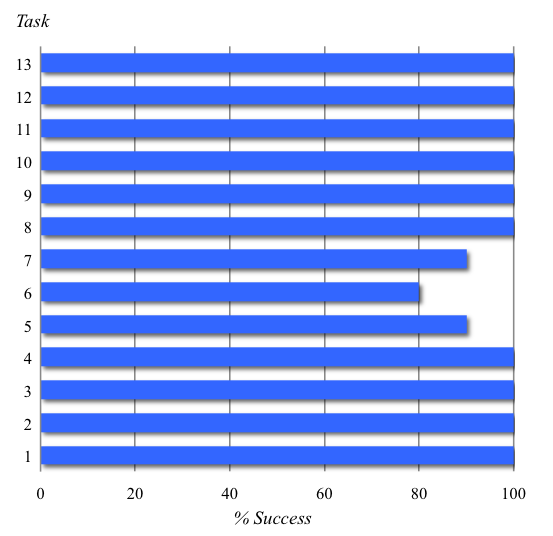
\includegraphics[scale=0.75]{img/tsuccess.png}} %[width=0.7\textwidth]
\caption{Representation of the percent of success for each task.}
\label{fig:tsuccess}   
\end{figure*}
The time it takes a participant to perform a task says a lot about the usability
of the application. In almost every situation, the faster a participant can
complete a task, the better the experience. In fact, it would be pretty unusual
for a user to complain that a task took less time than expected
\cite{albert2013measuring}.\\ Then, task-on-time was applied to measure time
that an user did the task. A resume of the time tasks for each user it is in
table \ref{tab:datausers}, \textit{null} values mean that the user didn't the task.
\begin{table}
\centering
\small
\caption{Time on task data for 10 users and 13 tasks. }
\label{tab:datausers}  
\begin{tabular}{lllllllllll}
\hline\noalign{\smallskip}
Task  & Us1  & Us2 & Us3 & Us4 & Us5 & Us6 & Us7 & Us8 & Us9 & Us10 \\
\noalign{\smallskip}\hline\noalign{\smallskip}
1 & 12  & 28 & 24 & 30 & 19 & 33  & 23 & 16 & 5  & 7 \\
2 & 3   & 4  & 17 & 5  & 17 & 134 & 9  & 16 & 12 & 11 \\
3 & 123 & 69 & 159& 53 & 69 & 113 & 44 & 41 & 70 & 98 \\
4 & 20  & 4  & 86 & 40 & 13 & 4   & 17 & 3  & 20 & 3 \\
5 & 50  & 10 & 63 & 50 & 7  & 11  & 10 & 5  & 20 & Null \\
6 & 10  & 30 & 28 & 27 & 5  & 46  & Null  & 7  & Null  & 34 \\
7 & 10  & 20 & 16 & 8  & 15 & Null & 9  & 24 & 16 & 28 \\
8 & 18  & 24 & 10 & 10 & 5  & 3   & 27 & 4  & 5  & 6 \\
9 & 5   & 6  & 31 & 4  & 45 & 9   & 12 & 5  & 3  & 8 \\
10 & 15 & 17 & 15 & 11 & 10 & 19  & 13 & 10 & 20 & 20 \\
11 & 30 & 15 & 20 & 16 & 20 & 22  & 15 & 13 & 18 & 20 \\
12 & 12 & 14 & 19 & 14 & 40 & 10  & 17 & 17 & 15 & 15 \\
13 & 25 & 15 & 15 & 14 & 10 & 10  & 11 & 10 & 10 & 25 \\
\noalign{\smallskip}\hline
\end{tabular}
\end{table}

\section{Results}

To measure the efficiency of the metric it was chose an confidence interval.  In
this way, it is observed the time variability within the same task and  also
helps visualize the difference across tasks to determine whether there is a
statistically significant difference between tasks. The obtained information is
in table \ref{tab:ic}, the median was used to calculate the confidence interval.
\begin{table}
\centering
\small
\caption{Confidence interval per task with a confidence level of 95\%. }
\label{tab:ic}    
\begin{tabular}{lllll}
\hline\noalign{\smallskip}
Task  & Median & CI 95\% & Upper bound & Lower bound  \\
\noalign{\smallskip}\hline\noalign{\smallskip}
1 &    20         & 5.96  & 25.96 & 14.04  \\
2 &    11.5      & 0.81  & 12.31  & 10.69   \\
3 &    69.5      &  25.57   &  95.07  &  43.93   \\
4 &    15        & 16.34  &  31.34  &  -1.34   \\
5 &    15.5     &  14.84  &  30.34  &  0.66  \\
6 &     27.5    &   11.57  &  39.07  &  15.93    \\
7 &     16       &  5.19  & 21.19  &  10.81   \\
8 &     8         &   5.80  &  13.80  & 2.20 \\
9 &     7         & 9.43  &  16.43  &  -2.43  \\
10 &   15       &   2.44  &  17.44   &  12.56   \\
11 &   19       &  3.00  &  22.00  &  16.00   \\
12 &   14.5    &  5.51  &  20.01  &  8.99   \\
13 &   12.5    &  3.89  &  16.39  &  8.61    \\
\noalign{\smallskip}\hline
\end{tabular}
\end{table}
In the next step the USE \textit{(Usefulnes, Satisfaction, and Ease of Use)}
questionnaire \cite{morris2001experience} was applied in order to get the user's
feedback and comments for to know about the difficults in the test.  The USE
questionnaire consists of 30 rating scales divided into 4 categories:
\textit{Usefulness, Satisfaction, Ease of Use, and Ease of Learning}. Each is a positive
statement to which the user rates level of agreement on a 7-point Likert scale.
The USE questionnaire(see appendix \ref{apendixb}) allows to get values for Usefulness, Satisfaction, Ease of Use, and Ease of Learning, the visualizing the results is in the
Fig.\ref{fig:radial} , where the four axis of the radar chart represent the
values of percent which users rated positively this factors with respect to
their interaction with the context-aware recommender system.  The accurate values are
\textit{Usability 83\%, Satisfaction 84\%, Easy of use  92\%, and Easy of Learning 81\%.}
\begin{figure*}
\centering
\small
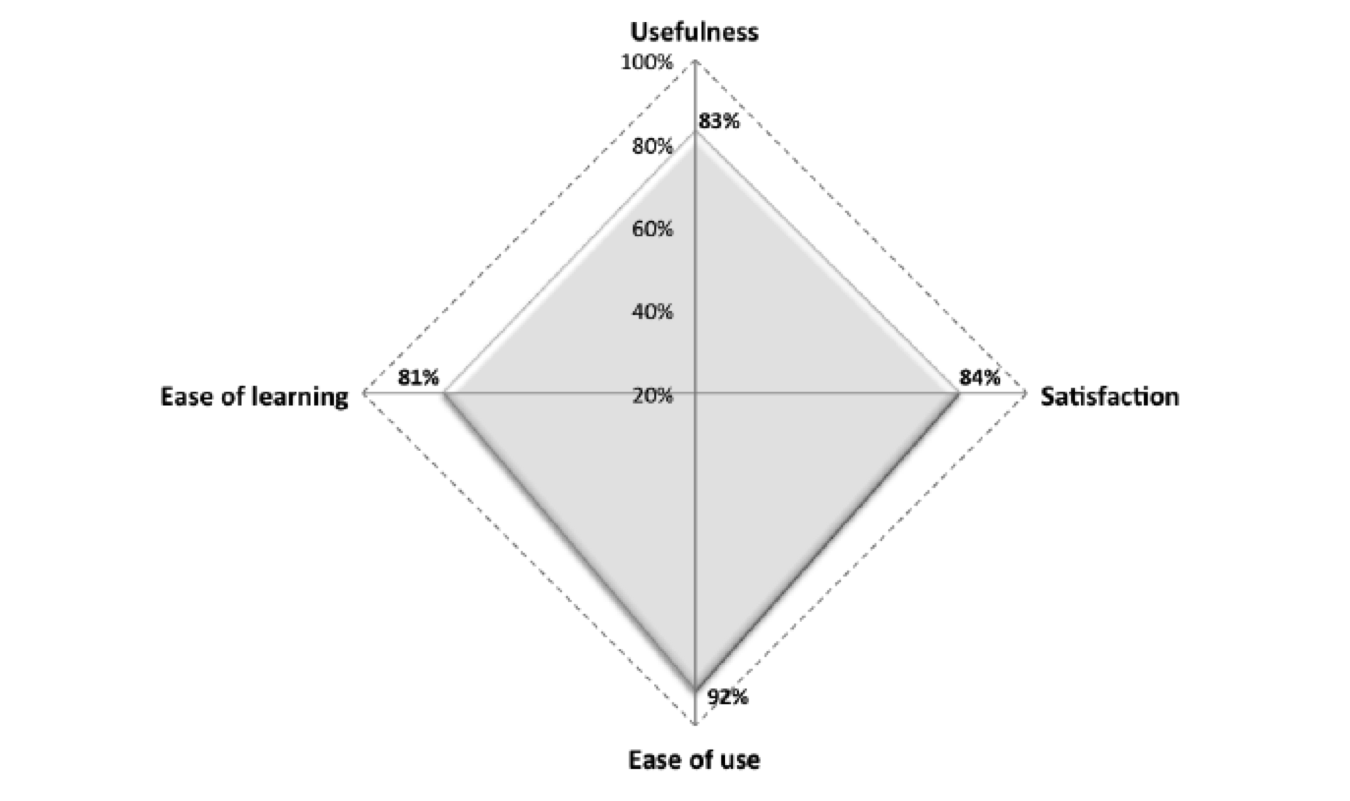
\includegraphics[width=0.8\textwidth]{img/radial.png}%[scale=0.5]{img/radial.png} 
\caption{\small{The radar chart that depicts the four axis evaluated in the questionnaire.}}
\label{fig:radial}   
\end{figure*}


